\section{最佳\texorpdfstring{$N$}{N}项逼近的误差}
\label{sec:besov-best-n-term}

上一节的截断对所有函数保留同一组坐标。若函数的大分量集中在少数几个位置，例如只在跳跃点附近有大的细尺度系数，预先固定的子空间就会把预算花在许多为零的分量上。本节保持同一周期正交小波基和$L^2$误差，改为允许每个函数跨组挑选至多$N$个分量。由第~\ref{chap:function-approximation}章的最大系数选择定理，最优的选择是保留绝对值最大的$N$个分量。

把粗项系数与全部细节系数排成一个序列，记它们的绝对值的非增重排为$c_1^*\geq c_2^*\geq\cdots$。由同一定理，最佳$N$项误差为
\begin{equation}
 \sigma_N(f)_2=\Bigl(\sum_{n>N}(c_n^*)^2\Bigr)^{1/2},
 \label{eq:besov-n-term-error}
\end{equation}
约定$\sigma_0(f)_2=\lVert f\rVert_2$。

为研究系数的集中程度怎样影响这个误差，本节取$0<s<1/2$，令
\begin{equation}
 \frac1\tau=s+\frac12,
 \label{eq:besov-tau}
\end{equation}
从而$1<\tau<2$，并研究$B^s_{\tau,\tau}$的系数条件。本节的函数都取自$L^2(\mathbb T)$，以便讨论$L^2$误差。

\subsection{跨尺度选择}
\label{sec:besov-adaptive-selection}

先看最极端的情形。取$f=\psi_{J',0}$，只有第$J'$组的一个分量非零。固定尺度截断在$J\leq J'$时还没有到达这一组，$E_J(f)=1$，遗漏全部能量，尽管已经用了$M_J=2^J$个基函数。最佳$N$项逼近在$N=1$时就保留这个分量，$\sigma_1(f)_2=0$。

贯穿的例子$f=\mathbf 1_{[0,1/3)}$更有代表性。它的坐标是$a_0=1/3$与每组一个的$2^{-j/2}/3$。按大小排列，$a_0$与第$0$组并列最大，之后是第$1,2,\ldots$组，于是前$N$项保留了$a_0$与第$0$组到第$N-2$组的非零分量。代入式~\eqref{eq:besov-n-term-error}，得到
\[
 \sigma_N(f)_2^2=\sum_{j\geq N-1}\frac{2^{-j}}{9}=\frac{2^{2-N}}{9},\qquad\sigma_N(f)_2=\frac23\,2^{-N/2}.
\]

$N$也取$8$，得到$\sigma_8(f)_2=1/24\approx0.0417$，是上一节$E_3(f)=1/6$的四分之一。图~\ref{fig:besov-haar-tiles}比较这两种选择：一个方格代表一个分量，上方的行是粗尺度。固定截断把$8$项用在前三层的全部方格上，其中一半的系数为零；最佳$N$项沿着跳跃点一路向下，每层只取一个方格。

\begin{BookInlineFigure}
  \centering
  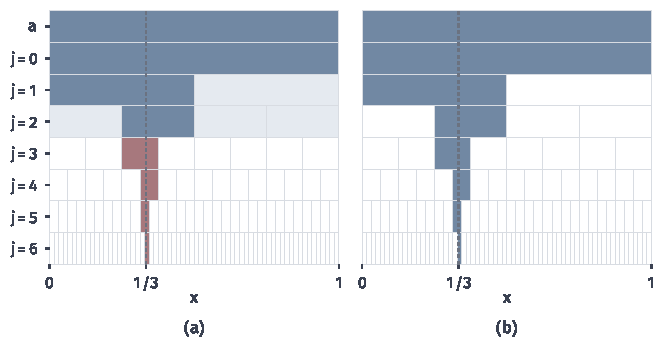
\includegraphics[width=112mm]{figures/04-spaces-measures-and-geometry/03-function-spaces/matplotlib/besov-haar-tiles/figure.pdf}
  \caption{$f=\mathbf 1_{[0,1/3)}$的Haar坐标，每个方格是一个基函数的位置和尺度，虚线标出跳跃点$x=1/3$。每层只有含跳跃点的方格系数非零。(a)固定尺度截断：浅蓝色是保留而系数为零的项，深蓝色是保留的非零项，红色是舍弃的非零项。(b)最佳$N$项：$N=8$项全部用在非零系数上。}
  \label{fig:besov-haar-tiles}
\end{BookInlineFigure}

两种做法的误差差别如表~\ref{tab:besov-fixed-vs-best}，图~\ref{fig:besov-error-decay}画出同样的数据。固定截断的误差按项数的$-1/2$次幂下降，最佳$N$项的误差按项数指数下降。

\begin{BookInlineTable}
  \centering
  \begin{tabular}{@{}cccccc@{}}
    \toprule
    项数 & $1$ & $2$ & $4$ & $8$ & $16$\\
    \midrule
    固定截断$E_J$（$M=2^J$） & $0.471$ & $0.333$ & $0.236$ & $0.167$ & $0.118$\\
    最佳$N$项$\sigma_N$ & $0.471$ & $0.333$ & $0.167$ & $0.042$ & $0.003$\\
    \bottomrule
  \end{tabular}
  \caption{$f=\mathbf 1_{[0,1/3)}$在Haar基下的两种误差。}
  \label{tab:besov-fixed-vs-best}
\end{BookInlineTable}

\begin{BookInlineFigure}
  \centering
  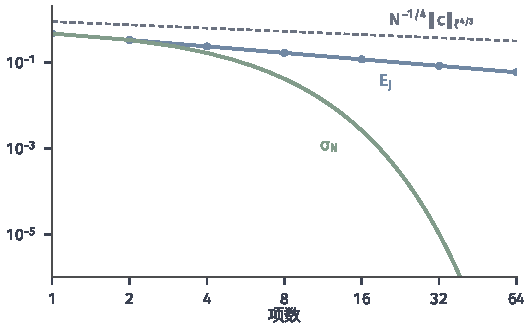
\includegraphics[width=90mm]{figures/04-spaces-measures-and-geometry/03-function-spaces/matplotlib/besov-error-decay/figure.pdf}
  \caption{同一函数的两种误差，双对数坐标。蓝色为固定截断$E_J$，圆点在$M=2^J$处；绿色为最佳$N$项误差$\sigma_N$；灰色虚线是定理~\ref{thm:besov-n-term-upper}在$s=1/4$时给出的上界。}
  \label{fig:besov-error-decay}
\end{BookInlineFigure}

换成更光滑的紧支撑小波，同样的现象仍然出现。设$\int\psi=0$。若$\psi_{j,k}$的支撑内部不含跳跃点，$f$在其上为常数，系数为零；含跳跃点的$k$每层只有有界个，并且
\[
 \lvert c_{j,k}\rvert\leq\lVert\psi_{j,k}\rVert_1=2^{-j/2}\lVert\psi\rVert_1 .
\]
所以每层只有有界个非零系数，大小按$2^{-j/2}$衰减，$\sigma_N$仍随$N$指数衰减。

固定截断则不然。阶跃函数不属于任何$s>1/2$的$B^s_{2,\infty}$，由定理~\ref{thm:besov-truncation-characterization}，$E_J(f)=O(2^{-Js})$对$s>1/2$不成立，用$M$个固定基函数的误差不能比$M^{-1/2}$快出一个幂次。

两种方式的差别在于保留哪些方向：固定截断按下标保留，自适应选择按大小保留。代价有两点。每个函数各自选择$N$个下标，要用有限个代表覆盖整个函数类时，还必须计入“选了哪些下标”这一信息。近似对$f$也不再是线性的：两个函数之和的最佳$N$项近似，一般不是各自近似之和。

\subsection{最佳\texorpdfstring{$N$}{N}项误差的上界}
\label{sec:besov-n-term-upper}

在$1/\tau=s+1/2$时，小波范数~\eqref{eq:besov-wavelet-norm}中$p=q=\tau$，权重$2^{j(s+1/2-1/\tau)}=1$完全抵消。组内和组间都用$\ell^\tau$，分组也就不再起作用：
\[
 \lVert f\rVert_{B^s_{\tau,\tau}}^{\mathrm w}=\lVert a\rVert_{\ell^\tau}+\Bigl(\sum_{j\geq j_0}\lVert c_j\rVert_{\ell^\tau}^\tau\Bigr)^{1/\tau}.
\]

记$c$为全部系数（包括有限个粗项）组成的序列。对非负数$A,B$有下面的比较：
\[
 (A^\tau+B^\tau)^{1/\tau}\leq A+B\leq2(A^\tau+B^\tau)^{1/\tau} .
\]
取$A=\lVert a\rVert_{\ell^\tau}$，$B$为细节部分的$\ell^\tau$范数，得到
\begin{equation}
 \lVert c\rVert_{\ell^\tau}\leq\lVert f\rVert^{\mathrm w}_{B^s_{\tau,\tau}}\leq2\lVert c\rVert_{\ell^\tau}.
 \label{eq:besov-ltau-coeff}
\end{equation}
所以$f\in B^s_{\tau,\tau}$恰好意味着全部系数$\tau$次可和，不再区分它们来自哪一层。

$\tau<2$时，$\ell^\tau$可和比平方可和更强。这与有限维中的现象相同：在单位$\ell^2$球面上，$\ell^\tau$范数小的向量大部分能量集中在少数分量上。表~\ref{tab:besov-concentrate-spread}中，$\tau=1$时集中的$c^{\mathrm A}$范数是$1$，分散的$c^{\mathrm B}$范数是$2^{3/2}$。

\begin{theorem}[最佳$N$项误差的上界]
\label{thm:besov-n-term-upper}
设$0<s<1/2$，$1/\tau=s+1/2$。则对每个$f\in L^2(\mathbb T)\cap B^s_{\tau,\tau}$和每个$N\geq1$，
\begin{equation}
 \sigma_N(f)_2\leq N^{-s}\lVert c\rVert_{\ell^\tau}\leq C_0N^{-s}\lVert f\rVert_{B^s_{\tau,\tau}} .
 \label{eq:besov-n-term-upper}
\end{equation}
\end{theorem}

\begin{proof}
重排序列的前$n$项都不小于$c_n^*$，所以$n(c_n^*)^\tau\leq\lVert c\rVert_{\ell^\tau}^\tau$，即
\[
 c_n^*\leq n^{-1/\tau}\lVert c\rVert_{\ell^\tau} .
\]

把式~\eqref{eq:besov-n-term-error}中每一项写成$(c_n^*)^2=(c_n^*)^{2-\tau}(c_n^*)^\tau$。$n>N$时$c_n^*\leq c_N^*$，于是
\[
 \sigma_N(f)_2^2\leq(c_N^*)^{2-\tau}\sum_{n>N}(c_n^*)^\tau\leq(c_N^*)^{2-\tau}\lVert c\rVert_{\ell^\tau}^\tau .
\]

代入$c_N^*$的上界，并用$(2-\tau)/\tau=2/\tau-1=2s$，得到
\[
 \sigma_N(f)_2^2\leq N^{-(2-\tau)/\tau}\lVert c\rVert_{\ell^\tau}^{2-\tau}\lVert c\rVert_{\ell^\tau}^\tau=N^{-2s}\lVert c\rVert_{\ell^\tau}^2 .
\]
第二个不等式由式~\eqref{eq:besov-ltau-coeff}与定理~\ref{thm:besov-wavelet-characterization}得到。
\end{proof}

用贯穿的例子核对。取$s=1/4$，则$\tau=4/3$。全部系数的$\ell^{4/3}$范数由几何级数给出：
\[
 \lVert c\rVert_{\ell^{4/3}}^{4/3}=3^{-4/3}\Bigl(1+\frac{1}{1-2^{-2/3}}\Bigr)\approx0.8557,\qquad\lVert c\rVert_{\ell^{4/3}}\approx0.890 .
\]
$N=8$时上界为$8^{-1/4}\times0.890\approx0.529$，实际误差$0.0417$远小于它。这个上界对整个球成立，它要照顾到最坏的函数，而这个例子的系数衰减得特别快。

图~\ref{fig:besov-parameter-map}把几个空间放到$(1/p,s)$平面上。竖线$p=2$上的点是上一节的$B^s_{2,q}$，球上的固定截断速率是$M^{-s}$。绿线上的点是$B^s_{\tau,\tau}$，球上的最佳$N$项速率是同样的$N^{-s}$。从竖线沿箭头移到绿线，速率不变，度量方式却换成了$\ell^\tau$：函数可以把大系数集中在少数位置，只要全部系数$\tau$次可和。

\begin{BookInlineFigure}
  \centering
  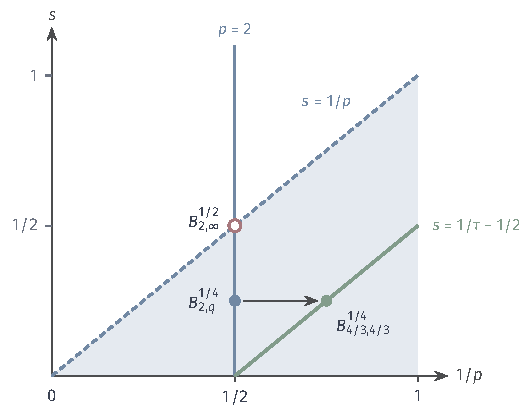
\includegraphics[width=90.1mm]{figures/04-spaces-measures-and-geometry/03-function-spaces/tikz/besov-parameter-map/figure.pdf}
  \caption{$(1/p,s)$平面上的Besov空间。蓝色竖线是$p=2$，绿线是$s=1/\tau-1/2$，箭头两端速率相同。虚线$s=1/p$是周期阶跃的临界线，其下方的浅蓝色区域内阶跃函数属于相应空间，红圈标出竖线上的临界点$B^{1/2}_{2,\infty}$。绿线整条位于浅蓝色区域内。}
  \label{fig:besov-parameter-map}
\end{BookInlineFigure}

图中还能读出阶跃函数为什么适合自适应逼近。在竖线上，阶跃函数的光滑阶数到$1/2$就停了。绿线却整条在临界线以下，因为$s=1/\tau-1/2<1/\tau$。在本节的范围$0<s<1/2$内，阶跃函数属于绿线上的每个空间。

\subsection{速率条件的逆向刻画}
\label{sec:besov-n-term-converse}

上界的反方向是：若误差满足$\sup_NN^s\sigma_N(f)_2<\infty$，函数是否属于$B^s_{\tau,\tau}$？答案是否定的，速率只对应一个更弱的条件。

\begin{theorem}[误差速率的刻画]
\label{thm:besov-n-term-rate}
设$s>0$，$1/\tau=s+1/2$，$f\in L^2(\mathbb T)$。则
\begin{equation}
 \sup_{N\geq1}N^s\sigma_N(f)_2<\infty\iff\sup_{n\geq1}n^{1/\tau}c_n^*<\infty .
 \label{eq:besov-n-term-rate}
\end{equation}
\end{theorem}

\begin{proof}
设$\sigma_N(f)_2\leq AN^{-s}$。第$N+1$到$2N$项共$N$项，都不小于$c_{2N}^*$，所以
\[
 N(c_{2N}^*)^2\leq\sum_{n=N+1}^{2N}(c_n^*)^2\leq\sigma_N(f)_2^2\leq A^2N^{-2s}.
\]
由此得到
\[
 c_{2N}^*\leq AN^{-s-1/2}=AN^{-1/\tau}.
\]
奇数下标用$c_{2N+1}^*\leq c_{2N}^*$，$n=1$用$c_1^*\leq\lVert f\rVert_2$，于是$\sup_nn^{1/\tau}c_n^*<\infty$。

反过来，设$c_n^*\leq Bn^{-1/\tau}$。代入式~\eqref{eq:besov-n-term-error}，用积分比较尾和，并用$2/\tau-1=2s>0$，得到
\[
 \sigma_N(f)_2^2\leq B^2\sum_{n>N}n^{-2/\tau}\leq B^2\int_N^\infty x^{-2/\tau}\,\mathrm dx=\frac{B^2N^{-2s}}{2s}.
\]
\end{proof}

条件$\sup_nn^{1/\tau}c_n^*<\infty$称为弱$\ell^\tau$条件，它比$\ell^\tau$可和弱。取$c_n^*=n^{-1/\tau}$，由$2/\tau=2s+1>1$，它平方可和，按任意次序放到基函数上就得到一个$L^2$函数$f$。它满足弱$\ell^\tau$条件，因而
\[
 \sigma_N(f)_2\leq(2s)^{-1/2}N^{-s}.
\]

可是$\sum_n(c_n^*)^\tau=\sum_nn^{-1}=\infty$，所以在$0<s<1/2$时$f\notin B^s_{\tau,\tau}$。单一的误差速率不能反推Besov成员资格，这与统一截断速率只对应$q=\infty$的情形相似。

\subsection{跨预算的误差汇总}
\label{sec:besov-approximation-spaces}

第~\ref{sec:besov-truncation-aggregation}小节看到，把截断误差跨尺度汇总可以恢复有限$q$的条件。对最佳$N$项误差也可以这样做：不只要求一个速率，而是把各个预算下的误差按$\ell^\tau$汇总。预算取二进值$N=2^m$。

\begin{definition}[逼近空间]
\label{def:besov-approximation-space}
设$s>0$，$1/\tau=s+1/2$。对$f\in L^2(\mathbb T)$，令
\begin{equation}
 \lVert f\rVert_{A^s_\tau}=\lVert f\rVert_2+\Bigl(\sum_{m\geq0}\bigl(2^{ms}\sigma_{2^m}(f)_2\bigr)^\tau\Bigr)^{1/\tau},
 \label{eq:besov-approximation-space}
\end{equation}
使其有限的函数组成的集合称为\term{逼近空间}（approximation space），记为$A^s_\tau$。
\end{definition}

$\sigma_N$随$N$单调不增，二进预算之间只差常数倍，所以$\sup_m2^{ms}\sigma_{2^m}(f)_2<\infty$等价于$\sup_NN^s\sigma_N(f)_2<\infty$。把上确界换成$\ell^\tau$和，正是把“统一速率”加强为“误差汇总”。

\begin{theorem}[逼近空间与Besov空间]
\label{thm:besov-approximation-equals-besov}
设$0<s<1/2$，$1/\tau=s+1/2$，小波满足定理~\ref{thm:besov-wavelet-characterization}的条件。则对$f\in L^2(\mathbb T)$，$f\in A^s_\tau$当且仅当$f\in B^s_{\tau,\tau}$，并且两个范数等价。
\end{theorem}

\begin{proof}
由式~\eqref{eq:besov-ltau-coeff}和定理~\ref{thm:besov-wavelet-characterization}，$\lVert f\rVert_{B^s_{\tau,\tau}}$与$\lVert c\rVert_{\ell^\tau}$等价，所以只需比较$\lVert f\rVert_{A^s_\tau}$与$\lVert c\rVert_{\ell^\tau}$。

先由系数控制误差汇总。由Parseval等式和$\tau<2$，$\lVert f\rVert_2$不超过$\lVert c\rVert_{\ell^\tau}$。把下标按二进块$2^l<n\leq2^{l+1}$分组，每块有$2^l$项，每项不超过$c_{2^l}^*$，所以
\[
 \sigma_{2^m}(f)_2^2\leq\sum_{l\geq m}2^l(c_{2^l}^*)^2 .
\]

记$\beta_l=2^{l/\tau}c_{2^l}^*$，则$2^l(c_{2^l}^*)^2=2^{-2ls}\beta_l^2$。乘以$2^{2ms}$并开方，得到
\[
 2^{ms}\sigma_{2^m}(f)_2\leq\Bigl(\sum_{l\geq m}2^{-2(l-m)s}\beta_l^2\Bigr)^{1/2}\leq\sum_{l\geq m}2^{-(l-m)s}\beta_l .
\]
由式~\eqref{eq:besov-convolution}，左端序列的$\ell^\tau$范数不超过$(1-2^{-s})^{-1}\lVert(\beta_l)\rVert_{\ell^\tau}$。

余下要用$\lVert c\rVert_{\ell^\tau}$控制$\lVert(\beta_l)\rVert_{\ell^\tau}$。$l\geq1$时，第$2^{l-1}+1$到$2^l$项共$2^{l-1}$项，都不小于$c_{2^l}^*$，所以
\[
 2^{l-1}(c_{2^l}^*)^\tau\leq\sum_{2^{l-1}<n\leq2^l}(c_n^*)^\tau .
\]
对$l$求和，并单独计入$\beta_0=c_1^*$，得到
\[
 \sum_{l\geq0}\beta_l^\tau\leq2\lVert c\rVert_{\ell^\tau}^\tau .
\]

再由误差汇总控制系数。下标$2^{m+1}\leq n<2^{m+2}$的块有$2^{m+1}$项，每项不超过$c_{2^{m+1}}^*$。由上一小节的论证，$2^m(c_{2^{m+1}}^*)^2\leq\sigma_{2^m}(f)_2^2$。所以
\[
 \begin{aligned}
 \sum_{n\geq2}(c_n^*)^\tau&\leq\sum_{m\geq0}2^{m+1}(c_{2^{m+1}}^*)^\tau\\
 &\leq2\sum_{m\geq0}2^{m(1-\tau/2)}\sigma_{2^m}(f)_2^\tau\\
 &=2\sum_{m\geq0}\bigl(2^{ms}\sigma_{2^m}(f)_2\bigr)^\tau ,
 \end{aligned}
\]
最后一步用了$\tau s=1-\tau/2$，它等价于$1/\tau=s+1/2$。

加上$c_1^*\leq\lVert f\rVert_2$，得到
\[
 \lVert c\rVert_{\ell^\tau}^\tau\leq\lVert f\rVert_2^\tau+2\lVert f\rVert_{A^s_\tau}^\tau .
\]
\end{proof}

这个定理说明，比统一速率更强的误差汇总恰好恢复了系数的强可和性。它依赖本节固定的条件：同一正交小波基，$L^2$误差，$1/\tau=s+1/2$，以及满足小波刻画条件的小波。换成冗余字典、其他误差范数或不匹配的指数，都需要另行分析。
